\documentclass[twoside,twocolumn]{article}

\usepackage{blindtext} 
\usepackage{graphicx}
\usepackage[sc]{mathpazo} 
\usepackage[T1]{fontenc} 
\linespread{1.05} 
\usepackage{microtype} 


\usepackage[english]{babel} 


\usepackage[hmarginratio=1:1,top=32mm,columnsep=20pt]{geometry} 
\usepackage[hang, small,labelfont=bf,up,textfont=it,up]{caption} 
\usepackage{booktabs} 


\usepackage{lettrine} 


\usepackage{enumitem} 
\setlist[itemize]{noitemsep} 


\usepackage{abstract} 
\renewcommand{\abstractnamefont}{\normalfont\bfseries} 
\renewcommand{\abstracttextfont}{\normalfont\small\itshape} 


\usepackage{titlesec} 
\renewcommand\thesection{\Roman{section}} % 
\renewcommand\thesubsection{\roman{subsection}} 
\titleformat{\section}[block]{\large\scshape\centering}{\thesection.}{1em}{} 
\titleformat{\subsection}[block]{\large}{\thesubsection.}{1em}{} 


\usepackage{fancyhdr} 
\pagestyle{fancy} 
\fancyhead{} 
\fancyfoot{} 
\fancyhead[C]{Modelo Dimensional vs Modelo Tabular$\bullet$ Octubre 2019 $\bullet$ } 
\fancyfoot[RO,LE]{\thepage} 


\usepackage{titling} 


\usepackage{hyperref} 


%----------------------------------------------------------------------------------------
%	TILULOS
%----------------------------------------------------------------------------------------


\setlength{\droptitle}{-4\baselineskip} 

\pretitle{\begin{center}\Huge\bfseries} 
\posttitle{\end{center}} 
\title{Modelo Dimensional vs Modelo Tabular} 
\author{Marko Antonio Rivas Rios\\  Jorge Luis Mamani Maquera\\ Edward Apaza Mamani
}
\date{\today} 
\renewcommand{\maketitlehookd}{


\noindent 
\begin{center}
Resumen
\end{center}
\textbf{}\\
El aumento de la cantidad de datos acumulados en las organizaciones ha provocado la aparición de nuevos requisitos de herramientas de análisis más complejas y eficientes, contexto en el cual la Business Intelligence surge como una disciplina para abordar este problema. La mejora de la eficiencia en el almacenamiento y el acceso a bases de datos analíticas ha sido reportada en muchas investigaciones, sobre las cuales varias compañías han introducido productos comerciales. Microsoft SQL Server 2017 ofrece dos alternativas independientes para crear modelos analíticos, el modelo multidimensional clásico y el modelo tabular más reciente. En este documento se realizó un análisis comparativo de ambos modelos, analizando profundamente sus características y potencialidades. 
\textbf{}\\

\noindent 
\begin{center}
Abstract 
\end{center}
\textbf{}\\
The increase in the amount of data accumulated in organizations has led to the emergence of new requirements for more complex and efficient analysis tools, a context in which business intelligence emerges as a discipline to address this problem. The improvement of storage efficiency and access to analytical databases has been reported in many investigations, on which several companies have used commercial products. Microsoft SQL Server 2017 offers two independent alternatives to create analytical models, the classic multidimensional model and the most recent tabular model. In this document a comparative analysis of both models was carried out, deeply analyzing their characteristics and potentialities.
}

%----------------------------------------------------------------------------------------

\begin{document}

% Print the title
\maketitle

%----------------------------------------------------------------------------------------
%	INTRODUCCION
%----------------------------------------------------------------------------------------

\section{Introduccion}
\lettrine[nindent=0em,lines=3]{A} la hora de definir nuestro modelo SSAS debemos analizar concienzudamente los diversos usos e implementaciones del que va a ser objeto el producto final, ya que aunque ambos tipos de elementos se creen en la herramienta de SSAS hay diferencias sustanciales, no que hagan que uno sea mejor y el otro peor si no que van encaminados a diferentes propósitos.

Una de la primeras y más importantes diferencias es que el motor de almacenamiento de los modelos tabulares es en memoria y persiste en disco, lo que garantiza su recuperación tras un reinicio.

Además su arquitectura permite que se generen modelos rápidamente ya que su implementación es sencilla y permite performance de rendimiento.

Los modelos tabulares están basados en columnas y no existe el concepto de agregaciones, lo que quiere decir, que cuando se realicen consultas sobre el mismo el motor de consulta solo trabajará con las columnas que figuren en la consulta.\textbf{}\\
Por último, en tabular no existe el concepto de “agregaciones” que existe en los cubos multidimensionales. El almacenamiento en los modelos tabulares está basado en columnas, esto es, que cuando se realiza una consulta MDX, el motor de consulta solo trabajará sobre las columnas especificadas en la consulta.
\textbf{}\\
Por otro lado tienen limitaciones,como que es no se permite más de una relación entre dos tablas, no se permiten relaciones muchos a muchos entre dos tablas o que para extraer datos del origen es necesario realizarlo mediante una única consulta por cada tabla del modelo.




%----------------------------------------------------------------------------------------
%	Objetivos
%----------------------------------------------------------------------------------------


\section{Objetivos}

\begin{itemize}
\item 

\textbf{Modelo Dimensional vs Modelo Tabular}
\\
\item Comprender las los modelos de forma dimensional y tabularl



\end{itemize}


%----------------------------------------------------------------------------------------
%	Marco teorico
%----------------------------------------------------------------------------------------


\section{Marco teorico}
\begin{enumerate}
\item \textbf{Modelo Dimensional }:\\
El modelo de datos dimensional, como ya se comentó en artículos anteriores, conlleva una técnica de modelado que facilita la compresión de la base de datos, haciéndola intuitiva para usuarios no expertos, y es comúnmente utilizada para implementar los DWH o DM.
Esta técnica goza de una gran aceptación y, a menudo, es elegida como la preferida para representar datos analíticos por cumplir simultáneamente con los siguientes requerimientos:\textbf{}\\
\textbf{}\\
- Dispone y estructura los datos de manera comprensibles para el usuario de negocio 
\textbf{}\\
- Genera un alto rendimiento en las búsquedas desde la capa de reporting
Dentro del modelado de datos dimensional destacan 2 conceptos clave: hechos y dimensiones.\textbf{}\\
\textbf{}\\
- Hechos: Son las métricas, normalmente valores cuantitativos (numéricos) susceptibles de ser agregados\textbf{}\\
\textbf{Ejemplo: }\\La cantidad de ventas de coches de un concesionario, el rendimiento en euros de una empresa, el número de estudiantes de un colegio, etc.\textbf{}\\
\textbf{}\\
- Dimensiones: Son los valores cualitativos. Proporcionan descripciones a los hechos, aportando un contexto a los mismos.\textbf{}\\
\textbf{Ejemplo: }\\Marca de coche, fecha, nombre concesionario, dirección de la empresa, nombre del colegio, etc.\textbf{}\\
\textbf{}\\
Existen 2 técnicas para llevar acabo el modelado dimensional: el esquema de estrella y el esquema de copo de nieve.
\textbf{}\\
\textbf{}\\
\textbf{Esquema de estrella}\\
Un esquema de estrella es un modelo de datos formado por una tabla de hechos, que contiene los datos para el análisis, rodeada de las tablas de dimensiones.

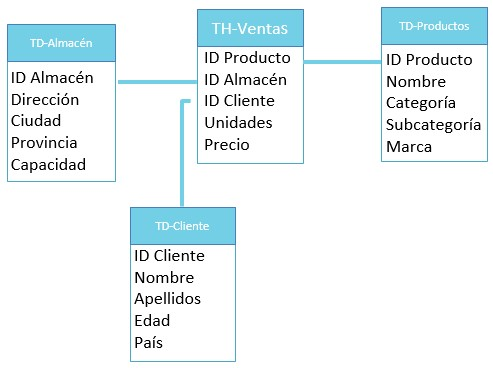
\includegraphics[width=7.5cm]{Imagenes/modelo2}

\textbf{}\\
Como podemos observar en la imagen 1 la tabla de hechos es TH-Ventas y está rodeada de las dimensiones TD-Almacén, TD-Producto y TD-Cliente, almacenando el ID de cada dimensión en la tabla de Hechos para, así, poder relacionar los atributos descriptivos de cada dimensión con la fila de la tabla de hechos.\textbf{}\\

El modelo estrella separa los datos del proceso de negocio en: hechos y dimensiones. Los hechos contienen datos medibles, cuantitativos, y las dimensiones los atributos que describen los datos indicados en los hechos.\textbf{}\\
\textbf{}\\
\textbf{Tabla de hechos}\\
- Clave principal compuesta por los claves principales de las tablas de dimensiones\\
\textbf{}\\
- Registra medidas o métricas de un evento específico. Ejemplo: cliente compra un geranio de maceta de 25cm en floristería mineral vegetal Lola a las 12:3 0am del 10 de Octubre de 2027\\
\textbf{}\\
- Evita repetir de manera completa los atributos dimensionales. En la TH sólo irá un ID de la dimensión\\
\textbf{}\\
- Se diseñan según el nivel de granularidad deseado, pudiendo registrar eventos a un gran nivel de atomicidad\\

\textbf{Tabla de dimensiones}\\
Tienen una clave primaria simple.\textbf{}\\

- Generalmente tienen un número bajo de registros\textbf{}\\
- Cada registro puede contener un gran número de atributos\textbf{}\\
- Suelen contener una surrogate primary key, generalmente una columna de tipo entero\textbf{}\\
\textbf{}\\
Las principales ventajas del esquema de estrella son:\textbf{}\\
- Queries simples. Las uniones y cruces son más sencillos, debido a su lógica, que los de un esquema normalizado\textbf{}\\
- Lógica de reporting simplificada\textbf{}\\
- Mejoras en el rendimiento de las consultas\textbf{}\\
- Agregaciones más rápidas. Gracias a las queries simplificadas\textbf{}\\
\textbf{}\\
Las principales desventajas del esquema de estrella son:\textbf{}\\
- Poco flexible. Los esquemas en estrella son construidos para una vista de los datos en particular


\textbf{Esquema en copo de nieve}\\
Un esquema de copo de nieve es una estructura más compleja que el esquema de estrella. Se da cuando alguna de las dimensiones se implementa con más de una tabla de datos.
El objetivo es normalizar estas tablas y reducir el espacio de almacenamiento al eliminar la redundancia.
Se representa como una tabla de hechos conectada con dimensiones anidadas. Al normalizar por completo las dimensiones el resultado parece un copo de nieve.\\
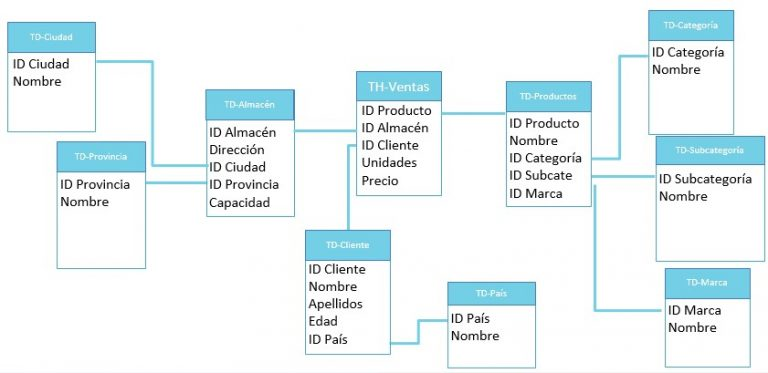
\includegraphics[width=7.5cm]{Imagenes/modelo3}
\textbf{}\\
Observamos en la imagen 2 como se dividen las dimensiones de TD-Almacén, TD-Producto y TD-Cliente en sub-dimensiones normalizadas.\textbf{}\\
\textbf{}\\
Las principales ventajas del esquema de copo de nieve son:\textbf{}\\

- Algunas herramientas de modelado de bases de datos multidimensional OLAP se optimizan\textbf{}\\
- La normalización de los atributos reduce el almacenamiento de datos\textbf{}\\
\textbf{}\\
\textbf{}\\

\textbf{}\\
\textbf{}\\
\textbf{}\\
Las principales desventajas del esquema de copo de nieve son:\textbf{}\\
- Queries complejas debido a la normalización (implica un mayor número de cruces)\textbf{}\\
- Bajo rendimiento debido a la normalización\textbf{}\\
\textbf{}\\
Después de haber descrito los esquemas de estrella y copo de nieve vamos a dejar una tabla con la comparativa entre los dos esquemas:

\textbf{}\\
\textbf{Beneficios del modelado dimensional}
\textbf{}\\
El modelado dimensional sigue siendo la técnica de modelado de datos más utilizada para diseñar almacenes de datos empresariales debido a los beneficios que produce. Éstos incluyen:
\textbf{}\\
\textbf{}\\
\textbf{Recuperación más rápida de datos}\\
El modelado dimensional combina las tablas en el propio modelo, lo que permite a los usuarios recuperar datos más rápido al ejecutar consultas de unión en comparación con los otros enfoques. El esquema desnormalizado de un modelo dimensional está optimizado para ejecutar consultas ad hoc. Como resultado, complementa en gran medida los objetivos de inteligencia empresarial (BI) de una organización.
\textbf{}\\
\textbf{}\\
\textbf{Mejor comprensión de los procesos de negocio}\\
La información en un modelo dimensional se almacena en tablas de hechos y dimensiones. Cubriremos qué hechos y dimensiones se encuentran en las secciones subsiguientes. Esta categorización de los datos en hechos y dimensiones, y la estructura entidad-relación de un modelo dimensional, presentan procesos de negocios complejos de una manera fácil de entender para los analistas.\textbf{}\\
\textbf{}\\
\textbf{}\\

\textbf{Flexible para cambiar}\\
El marco de modelado dimensional hace que el diseño del almacén de datos sea extensible. El diseño se puede modificar fácilmente para incorporar nuevos requisitos comerciales o realizar ajustes. Se pueden agregar nuevas entidades en el modelo o se puede cambiar el diseño de las existentes para reflejar los procesos comerciales modificados.
\textbf{}\\
\textbf{}\\
\textbf{Apartir de aqui es tu parte marko xd}\\
\item \textbf{ Modelo Tabular}: se utiliza para la construcción de un almacén de datos (data warehouse, DW) es decir, una colección de datos situada en un determinado lugar, (empresa, organización, etc.), integrado y variable en el tiempo, ayudando a la toma de decisiones. (Inestroza, 2018) \\

\textbf{Enfoque Kimball}
\\ \\
Contiene varios principios básicos que se analizan detenidamente en el libro de herramientas de Data Warehouse Lifecycle, Second Edition (Kimball, Ross, Mundy, y Becker, 2008)
\begin{itemize}
\item Seguir una metodología comprobada como el  ciclo de vida Kimball.
\item Comprender los requisitos comerciales para priorizar esfuerzos y generar valor comercial. 
\item Diseñar los conjuntos de datos con las características de usabilidad, flexibilidad y rendimiento.
\item Crear y entregar con rapidez los incrementos de los datos basados en procesos comerciales, conocidos con el nombre de almacenamiento de datos. 
\item Diseñar y construir una arquitectura de sistema DW/BI basado en lo que el negocio necesite, según su volumen de datos y entorno de sistemas de TI. 
\item Desarrollar el sistema de extracción, transformación y carga (ETL) con componentes estándar que se encuentran en el entorno de datos analíticos para tratar los patrones de diseño comunes.
\item Brindar la información total, tales como: informes, herramientas de consulta, aplicaciones, portales, documentación, capacitación y soporte.
\end{itemize}



\textbf{Business dimensional lifecycle}
\\ \\
La metodología se basa en lo que Kimball denomina, traducida al español “Ciclo de Vida Dimensional del Negocio”. Basado en cuatro principios básicos:

\begin{itemize}
\item Centrarse en el negocio.
\item Construir una infraestructura de información adecuada.
\item Realizar entregas en incrementos significativos (este principio consiste en crear el almacén de datos (DW) en incrementos entregables en plazos de 6 a 12 meses, en este punto, la metodología se parece a las metodologías ágiles de construcción de software).
\item Ofrecer la solución completa (En este se punto proporcionan todos los elementos necesarios para entregar valor a los usuarios de negocios, para esto ya se debe tener un almacén de datos bien diseñado, se deberán entregar herramientas de consulta ad hoc, aplicaciones para informes y análisis avanzado, capacitación, soporte, sitio web y documentación).

\end{itemize}
La construcción de una solución de DW/BI (Datawarehouse/Business Intelligence) es sumamente compleja, y Kimball plantea una metodología que simplifica esa complejidad. \\ \\
El enfoque del ciclo de vida Kimball se ilustra en el siguiente diagrama. Facilita una hoja de ruta general que constituye la serie de tareas de alto nivel solicitadas para proyectos exitosos de DW / BI.


\includegraphics[width=7.5cm]{Imagenes/Kimboll2}

\textit{"Independientemente de los objetivos específicos de DW / BI de su organización, creemos que un objetivo global del equipo debería ser la aceptación comercial de los entregables de DW / BI para respaldar la toma de decisiones de la empresa. Este objetivo debe permanecer a la vanguardia en todo el diseño, desarrollo e implementación de su sistema DW / BI "} (Arias, 2018)
\\ \\


\textbf{Definicion de requerimientos}

Entre las tareas para definir los requerimientos, existe una flecha bidireccional, esta indica que los requerimientos del negocio son el soporte inicial y también tiene influencia en el plan del proyecto.\\

Si nos fijamos en el centro del diagrama, vemos las tareas asociadas al área de “Datos”, en esta, se diseña e implementa el modelo dimensional, se desarrolla el sub-sistema de extracción, transformación, carga (extract, transformation, and Load-ETL) \\

Las tareas pertenecientes a esta área son:

\begin{itemize}
\item [1.] Modelado Dimensional
\begin{itemize}
\item [1.1.] Elección del proceso de negocio
\item [1.2.] Establecer el nivel de granularidad
\item [1.3.] Elegir las dimensiones
\item [1.4.] Identificar medidas y las tablas de hechos
\end{itemize}
\item [2.] Diseño Físico
\item [3.] Diseño e Implementación del subsistema de Extracción, Transformación y Carga (ETL)
\item [4.] Implementación
\item [5.] Mantenimiento y Crecimiento del Data Warehouse
\textbf{}\\
\textbf{}\\
\item \textbf{Inmon vs Kimball}: \\

Si recordamos lo expuesto en entradas anteriores, el datawarehouse de Kimball está orientado a la consulta de la información, por lo que su estructura interna está especialmente diseñada para garantizar una explotación de los datos rápida y sencilla, no requiriendo usuarios especializados para ello. Por el contrario, el datawarehouse de Inmon persigue la integración de todos los datos de la compañía, estando orientado hacia el almacenaje de grandes volúmenes de datos, por lo que su estructura interna normalizada se diseña para evitar la redundancia de datos, simplificar las labores de mantenimiento, etc. cuestiones que complican las consultas de la información, requiriendo que los usuarios finales estén mucho más especializados. \\
Así, podríamos decir que el enfoque de Kimball se ajusta más a proyectos pequeños en los que se persiga un sistema fácilmente explotable y entendible por el usuario y de rápido desarrollo, siendo el modelo de Inmon más apropiado para sistemas complejos de mayor envergadura. \\
Todo proyecto tiene sus propias peculiaridades, siendo cada caso único e independiente, por lo que resulta necesario llevar a cabo un estudio de todas ellas antes de decantarnos por una solución u otra, de forma que podamos hacernos una idea sobre qué modelo se ajusta mejor a las condiciones de nuestro proyecto. \\
Aun así, tampoco debemos cerrarnos a estas dos opciones, ya que existen casos en los que se han implantado soluciones intermedias entre ambas visiones, logrando así sistemas híbridos que permiten conjugar con éxito las ventajas de ambas perspectivas. \\

\end{itemize}


	
\end{enumerate}





%----------------------------------------------------------------------------------------
%	Ejemplo
%----------------------------------------------------------------------------------------


%----------------------------------------------------------------------------------------
%	Análisis
%----------------------------------------------------------------------------------------





%----------------------------------------------------------------------------------------
%	CONCLUSIONES
%----------------------------------------------------------------------------------------

\section{Conclusiones}
\begin{itemize}	
\item
Se ha demostrado que tanto el enfoque de Inmon como el de Kimball funcionan para entregar con éxito almacenes de datos. Incluso hay organizaciones donde se ha implementado una combinación de ambos ('modelo híbrido'). En un modelo híbrido, el almacén de datos se construye utilizando el modelo Inmon, y además del almacén de datos integrado, los almacenes de datos orientados a procesos de negocio se construyen utilizando el esquema en estrella para la presentación de informes. No podemos generalizar y decir que un enfoque es mejor que el otro; Ambos tienen sus ventajas y desventajas, y ambos funcionan bien en diferentes escenarios. El arquitecto tiene que seleccionar un enfoque para el almacén de datos en función de los diferentes factores; Se identificaron algunas claves en este documento. Finalmente, para que cualquier enfoque sea exitoso, debe ser cuidadosamente pensado, discutido en detalle.
\end{itemize} 



%----------------------------------------------------------------------------------------
%	BIBLIOGRAFIA
%----------------------------------------------------------------------------------------


\begin{thebibliography}{99} 

\bibitem[1]{}
\newblock Arias, D. (4 de marzo de 2018). Todo Sobre La Metodologia Kimball. Obtenido de postparaprogramadores: https://postparaprogramadores.com/metodologia-kimball

\bibitem[2]{}
\newblock Inestroza, M. (18 de Junio de 2018). METODOLOGÍA KIMBALL. Obtenido de goconsultores.com: http://www.goconsultores.com/tag/metodologia-kimball/

\bibitem[3]{}
\newblock Kimball, R., Ross, M., Mundy, J., \& Becker, B. (2008). The Data Warehouse Lifecycle Toolkit, 2nd Edition. Wiley.

\bibitem[4]{}
\newblock Inmon, WH  Construyendo el Data Warehouse, cuarta edición . John Wiley \& Sons., 2005.
\bibitem[5]{}
\newblock Marakas, George M.  Almacenamiento moderno de datos, minería y visualización . Prentice Hall, 2003.
\bibitem[6]{}
\newblock Kimball, Ralph y Margy Ross. The Data Warehouse Toolkit: The Definitive Guide to Dimensional Modeling, Third Edition . John Wiley \& Sons. 2013. Libros 24x7.
\bibitem[7]{}
\newblock Zentut 2016. "Arquitectura del almacén de datos Ralph Kimball" Zentut . com . Consultado el 25 de mayo de 2016. 
\bibitem[8]{}
\newblock Inmon, WH 2010. “UNA CUENTA DE DOS ARQUITECTURAS”
\bibitem[9]{}
\newblock Stanford 2003. "Conceptos de almacenamiento de datos" Stanford.edu. Consultado el 26 de mayo de 2016.

\end{thebibliography}


%----------------------------------------------------------------------------------------


\end{document}
